\documentclass{article}

% Paquetes (estilo base de la plantilla de Overleaf)
\usepackage[T1]{fontenc}
\usepackage[spanish,es-tabla,es-noquoting,es-nodecimaldot]{babel}
\usepackage{csquotes}
\usepackage[letterpaper,top=2cm,bottom=2cm,left=3cm,right=3cm,marginparwidth=1.75cm]{geometry}
\usepackage{amsmath}
\usepackage{graphicx}
\usepackage{booktabs}
\usepackage{tabularx}
\usepackage{float}
\usepackage[section]{placeins}
\usepackage[colorlinks=true, allcolors=blue]{hyperref}
\usepackage[backend=biber, style=authoryear]{biblatex}
\addbibresource{references.bib}

\title{Clasificación supervisada de coberturas tras el colapso de la presa de Brumadinho (Minas Gerais, Brasil) con Sentinel-2\\[0.5em]
\large Proyecto final -- Fase 1: definición del problema}
\author{Jose Villarroel, Jose D. Medina, Camila Beltrán y Juan Rodríguez\\Pontificia Universidad Javeriana}
\date{\today}

\begin{document}

\maketitle

\begin{abstract}
Este documento presenta la primera fase de un análisis comparativo de arquitecturas de aprendizaje automático para la clasificación de coberturas terrestres con imágenes satelitales. Se define el evento de estudio, el colapso de la presa I de la mina Córrego do Feijão el 25 de enero de 2019, y se delimita un área de 74{,}2\,km$^2$ en Brumadinho (Brasil). Se describe la escena Sentinel-2 L2A del 1 de febrero de 2019, de la que se usan las doce bandas espectrales remuestreadas a 10\,m. Por último, se documenta la construcción del conjunto de entrenamiento: 88 polígonos distribuidos en seis clases de cobertura, de los que se extraen 1640 píxeles con sus coordenadas, sus valores espectrales y su etiqueta en un archivo TSV.
\end{abstract}

\section{Introducción}
El proyecto final compara cinco arquitecturas de aprendizaje automático para clasificar las coberturas terrestres de una escena satelital multiespectral: regresión logística, árboles de decisión, máquinas de soporte vectorial, redes neuronales artificiales y un quinto modelo (KNN o Naive Bayes). El flujo de trabajo es el de una aplicación de GeoAI. Primero, los píxeles de la imagen se transforman en una tabla. Luego se entrenan y evalúan los modelos sobre esa tabla. Finalmente, el mejor modelo se aplica de nuevo al ráster completo para obtener un mapa temático y el área de cada clase.

Esta primera entrega corresponde a la fase de definición del problema y contiene cuatro partes:
\begin{enumerate}
 \item el evento elegido;
 \item los límites del área de estudio;
 \item los metadatos de la imagen satelital;
 \item la creación del conjunto de datos de entrenamiento.
\end{enumerate}
El procesamiento se realizó con scripts de Python basados en \texttt{rasterio} \parencite{GDAL}, sin depender de un sistema de información geográfica. QGIS \parencite{QGIS_Software} se utilizó únicamente para visualizar los resultados y revisar los polígonos.

\section{Evento seleccionado}
Se retoma el caso del proyecto de mitad de semestre: el colapso de la presa I de la mina Córrego do Feijão, en Brumadinho (Minas Gerais, Brasil), ocurrido el 25 de enero de 2019. La rotura liberó cerca de 12 millones de m$^3$ de relaves de mineral de hierro. El flujo de lodo cubrió el valle del Ribeirão Ferro-Carvão, sepultó instalaciones de la mina, viviendas y áreas agrícolas, y alcanzó el río Paraopeba \parencite{Rotta2020}.

En el proyecto de mitad de semestre el evento se abordó como un problema de detección de cambios entre dos fechas, mediante los índices NDVI y NDWI. En este proyecto la pregunta es otra: qué coberturas hay en el área una semana después del desastre y qué superficie ocupa cada una. Por esta razón se utiliza una única escena posterior al evento, la del 1 de febrero de 2019, que corresponde a la fecha $t_2$ del trabajo anterior. En ella el relave depositado aparece como una cobertura propia, con una firma espectral distinta de la del suelo expuesto de la mina, de la vegetación y del agua. Esto permite tratarlo como una clase y cuantificar su extensión en el mapa final.

\section{Área de estudio}
El área de estudio es la misma ventana empleada en el proyecto de mitad de semestre (Figura~\ref{fig:area}). Se ubica al suroeste de Belo Horizonte, en el Cuadrilátero Ferrífero. Su relieve es ondulado, con un mosaico de bosque atlántico, pastos, zonas urbanas y explotaciones mineras de hierro. Dentro del área se encuentran la mina Córrego do Feijão (al noreste), el corredor del relave a lo largo del Ribeirão Ferro-Carvão, el casco urbano de Brumadinho (al suroeste) y el tramo del río Paraopeba que lo atraviesa. La Tabla~\ref{tab:limites} resume sus límites.

\begin{table}[htbp]
 \centering
 \caption{Límites del área de estudio.}
 \label{tab:limites}
 \begin{tabularx}{\textwidth}{lX}
  \toprule
  Parámetro & Valor \\
  \midrule
  Longitud (WGS84) & $-44{,}224111^\circ$ a $-44{,}096943^\circ$ \\
  Latitud (WGS84) & $-20{,}159193^\circ$ a $-20{,}108763^\circ$ \\
  Área del rectángulo & 74{,}19\,km$^2$ medida en UTM 23S (74{,}61\,km$^2$ según Copernicus Browser) \\
  Extensión del ráster (UTM 23S) & E 581\,040--594\,420\,m; N 7\,770\,600--7\,776\,300\,m \\
  Dimensiones del ráster & $1338 \times 570$ píxeles de 10\,m ($13{,}38 \times 5{,}70$\,km) \\
  Sistema de referencia & WGS 84 / UTM zona 23S (EPSG:32723) \\
  Archivos & \texttt{study\_area.gpkg} (área) y \texttt{ROI\_Brumadinho.gpkg} (corredor) \\
  \bottomrule
 \end{tabularx}
\end{table}

La extensión del ráster es la envolvente del rectángulo geográfico proyectado a UTM, ajustada a la malla de 60\,m de Sentinel-2 para que todas las bandas compartan exactamente la misma retícula. El polígono del corredor del relave, delimitado en el trabajo anterior, se conserva como capa de apoyo. No restringe la clasificación, que cubre todo el rectángulo, pero se utiliza para ubicar las muestras de la clase relave minero.

\begin{figure}[htbp]
 \centering
 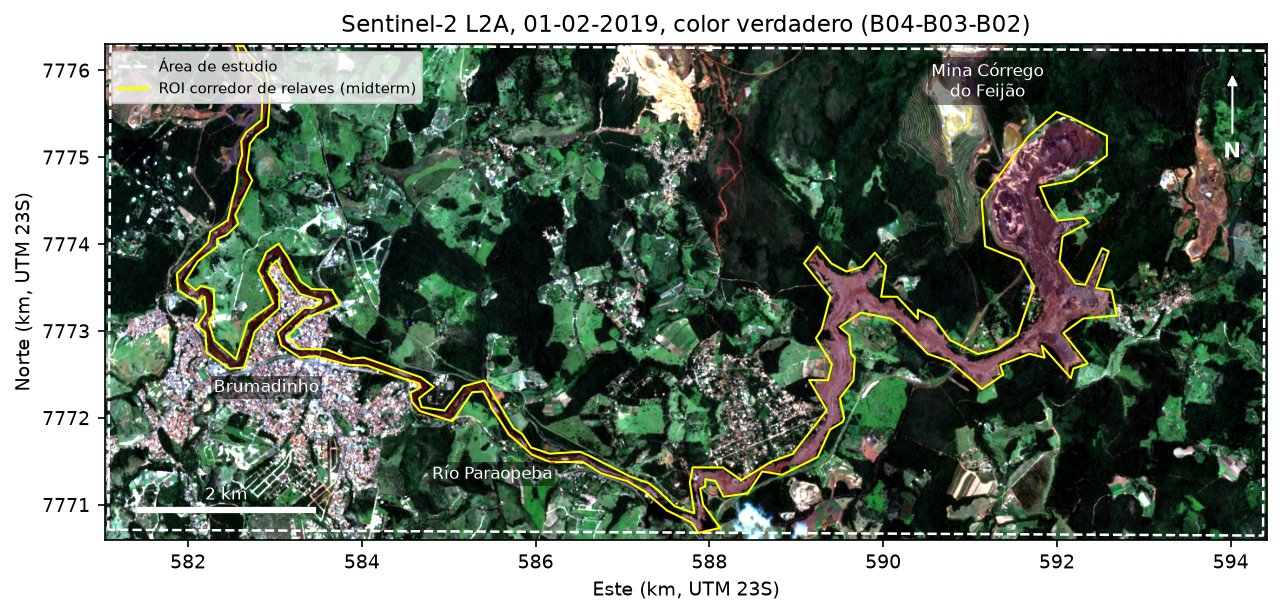
\includegraphics[width=\textwidth]{figures/area_estudio_tc}
 \caption{Área de estudio (línea blanca discontinua) y corredor del relave (amarillo) sobre la escena Sentinel-2 del 1 de febrero de 2019 en color verdadero.}
 \label{fig:area}
\end{figure}

\section{Imagen satelital}

\subsection{Selección y adquisición}
La escena se buscó en el catálogo STAC de Microsoft Planetary Computer \parencite{PlanetaryComputer}, en la colección \texttt{sentinel-2-l2a}. El criterio fue que la escena fuera del 1 de febrero de 2019 y cubriera por completo el área de estudio, y solo una cumplió ambas condiciones. Es la misma adquisición del satélite Sentinel-2A usada en el trabajo anterior; sus metadatos se resumen en la Tabla~\ref{tab:meta}.

Se cambió la fuente de descarga, que antes era Copernicus Browser, porque este proyecto exige al menos diez bandas. El catálogo STAC permite leer las doce bandas directamente desde archivos \emph{Cloud-Optimized GeoTIFF} y descargar solo la ventana del área de estudio.

\begin{table}[htbp]
 \centering
 \small
 \caption{Metadatos de la escena utilizada.}
 \label{tab:meta}
 \begin{tabularx}{\textwidth}{lX}
  \toprule
  Campo & Valor \\
  \midrule
  Identificador del producto & \texttt{S2A\_\allowbreak{}MSIL2A\_\allowbreak{}20190201T131241\_\allowbreak{}N0212\_\allowbreak{}R138\_\allowbreak{}T23KNT\_\allowbreak{}20201007T130407.SAFE} \\
  Plataforma / sensor & Sentinel-2A / MSI \\
  Nivel de procesamiento & L2A (Sen2Cor), reflectancia BOA \\
  \emph{Processing baseline} & 02.12 \\
  Fecha y hora de adquisición (UTC) & 2019-02-01 13:12:41 \\
  Tile MGRS / órbita relativa & 23KNT / R138 (descendente) \\
  Nubosidad de la escena completa & 1{,}14\,\% \\
  Píxeles inválidos (SCL) en el área & 0{,}11\,\% \\
  Ángulos solares medios & cenital 27{,}1$^\circ$, azimut 87{,}8$^\circ$ \\
  SRC del stack & WGS 84 / UTM zona 23S (EPSG:32723) \\
  Tamaño de píxel & 10\,m $\times$ 10\,m \\
  Dimensiones & 1338 columnas $\times$ 570 filas \\
  Tipo de dato / escala & UInt16, reflectancia $\times$ 10\,000 (sin offset) \\
  Fuente & Microsoft Planetary Computer (STAC, \texttt{sentinel-2-l2a}) \\
  \bottomrule
 \end{tabularx}
\end{table}


El producto es de nivel 2A, es decir, reflectancia en la superficie (BOA) corregida atmosféricamente con Sen2Cor \parencite{MainKnorn2017}. En la versión de procesamiento 02.12 no se aplica un desplazamiento radiométrico, por lo que la reflectancia se obtiene como $\rho = DN / 10\,000$.

\subsection{Bandas espectrales}
Se emplearon las doce bandas disponibles en el nivel L2A, listadas en la Tabla~\ref{tab:bandas}. La banda B10, de cirros, solo existe en el nivel L1C. Las bandas de 20 y 60\,m se remuestrearon a 10\,m por interpolación bilineal. Las bandas de 10\,m conservan sus valores originales, porque la malla de salida coincide con la nativa. El resultado es un único GeoTIFF de doce bandas en formato UInt16, que se usa tanto para extraer el conjunto de entrenamiento como para la inferencia de la Fase~3.

\begin{table}[htbp]
 \centering
 \caption{Bandas Sentinel-2 L2A utilizadas \parencite{Drusch2012}.}
 \label{tab:bandas}
 \begin{tabular}{llrrl}
  \toprule
  Banda & Región & $\lambda$ central (nm) & Res. nativa (m) & Remuestreo \\
  \midrule
  B01 & Aerosol costero & 443 & 60 & Bilineal a 10 m \\
  B02 & Azul & 490 & 10 & --- \\
  B03 & Verde & 560 & 10 & --- \\
  B04 & Rojo & 665 & 10 & --- \\
  B05 & Borde rojo 1 & 705 & 20 & Bilineal a 10 m \\
  B06 & Borde rojo 2 & 740 & 20 & Bilineal a 10 m \\
  B07 & Borde rojo 3 & 783 & 20 & Bilineal a 10 m \\
  B08 & NIR & 842 & 10 & --- \\
  B8A & NIR estrecho & 865 & 20 & Bilineal a 10 m \\
  B09 & Vapor de agua & 945 & 60 & Bilineal a 10 m \\
  B11 & SWIR 1 & 1610 & 20 & Bilineal a 10 m \\
  B12 & SWIR 2 & 2190 & 20 & Bilineal a 10 m \\
  \bottomrule
 \end{tabular}
\end{table}


\subsection{Control de calidad}
La capa de clasificación de escena (SCL) se descargó sobre la misma malla, remuestreada por vecino más cercano. Se consideran inválidos los píxeles de las clases 0, 1, 3, 8, 9 y 10: sin datos, saturados, sombra de nube, nubes de probabilidad media y alta, y cirros. Estos píxeles representan el 0{,}11\,\% del área (Figura~\ref{fig:scl}) y se excluyen del conjunto de datos.

La Figura~\ref{fig:fc} presenta dos composiciones en falso color. En ambas el relave se distingue con claridad de la vegetación y del suelo expuesto de la mina.

\begin{figure}[htbp]
 \centering
 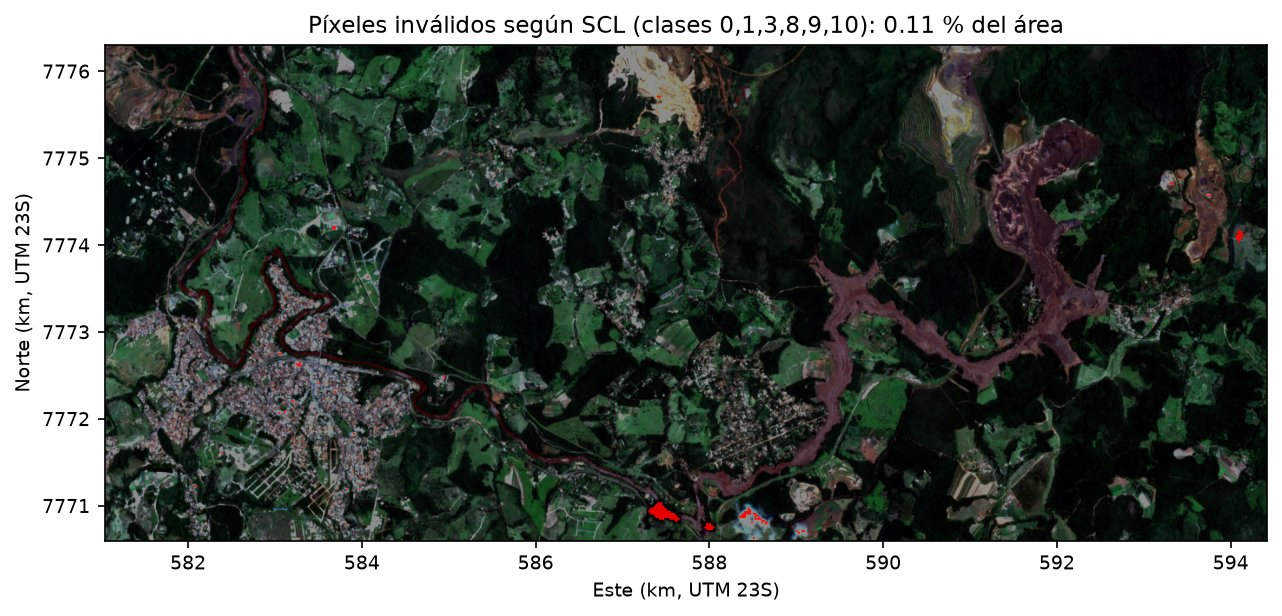
\includegraphics[width=0.9\textwidth]{figures/scl_mask}
 \caption{Píxeles inválidos según la banda SCL, en rojo.}
 \label{fig:scl}
\end{figure}

\begin{figure}[htbp]
 \centering
 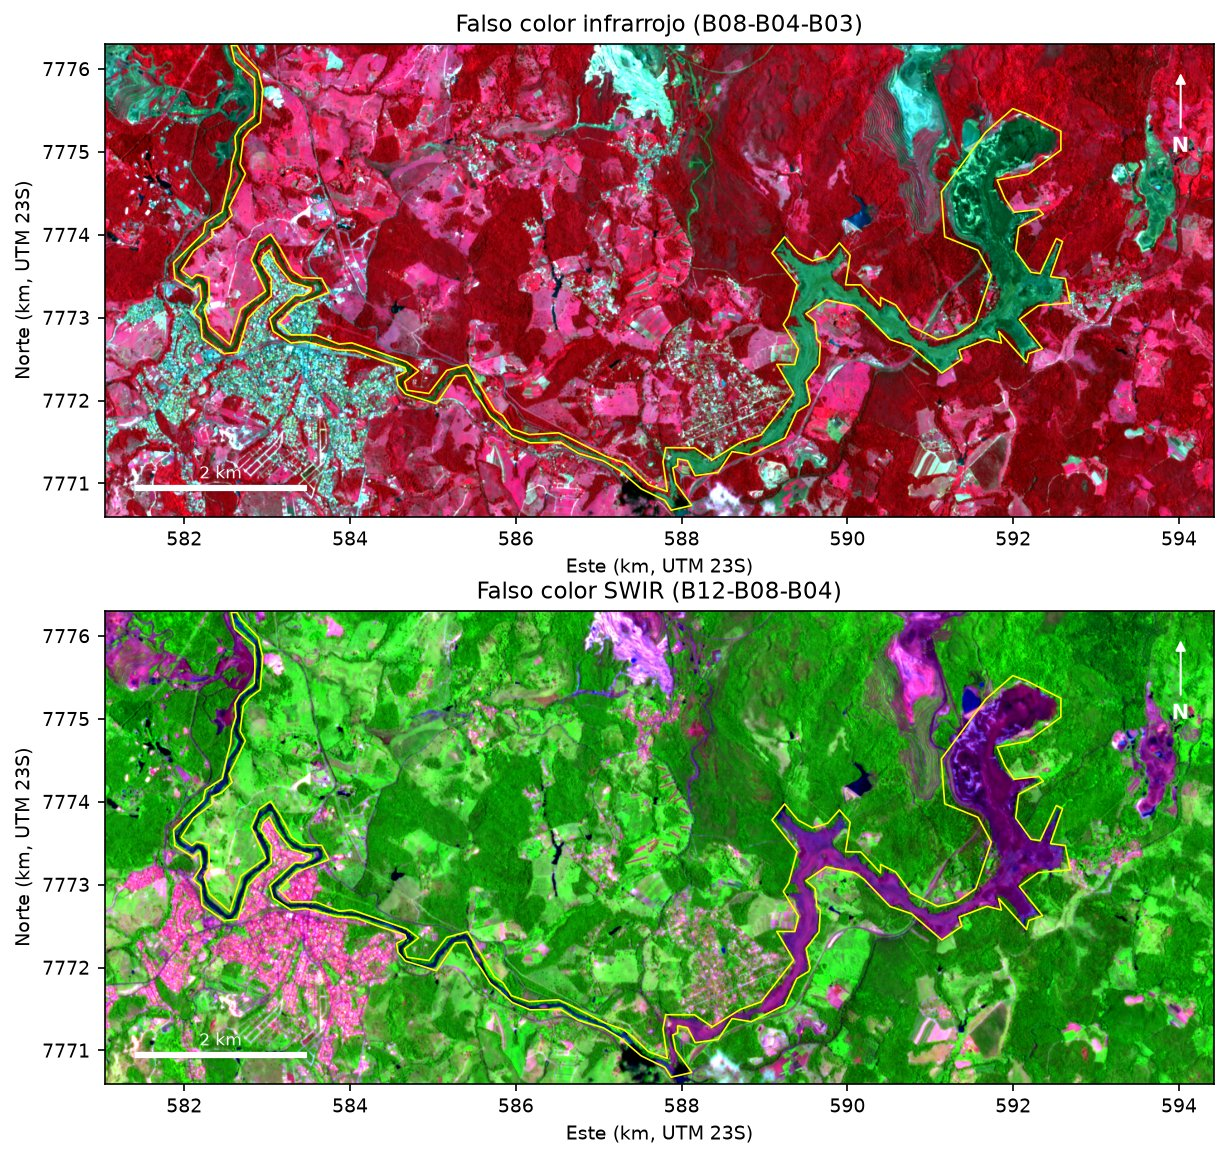
\includegraphics[width=0.9\textwidth]{figures/falso_color}
 \caption{Composiciones en falso color. Arriba, infrarrojo (R=B08, G=B04, B=B03): la vegetación aparece en rojo y el relave en verde oscuro. Abajo, SWIR (R=B12, G=B08, B=B04): el suelo expuesto y las zonas urbanas resaltan en tonos claros.}
 \label{fig:fc}
\end{figure}

\section{Creación del conjunto de datos}

\subsection{Esquema de clases}
Se definieron seis clases de cobertura a partir de la interpretación visual de la escena y de los objetivos del proyecto (Tabla~\ref{tab:clases}). El código numérico de cada clase será el valor del píxel en el ráster temático final.

\begin{table}[htbp]
 \centering
 \caption{Clases de cobertura.}
 \label{tab:clases}
 \begin{tabularx}{\textwidth}{clX}
  \toprule
  Código & Clase & Descripción \\
  \midrule
  1 & Vegetación densa & Bosque atlántico y vegetación arbórea, con NDVI muy alto y SWIR bajo. \\
  2 & Vegetación baja & Pastos, cultivos y vegetación herbácea, con NDVI medio-alto y SWIR alto. \\
  3 & Agua & Cuerpos de agua abiertos: lagunas de la mina y cauces. \\
  4 & Relave minero & Lodo de mineral de hierro depositado por el colapso en el valle del Ribeirão Ferro-Carvão. \\
  5 & Suelo expuesto & Tajos y pilas de la minería, vías sin pavimentar y suelo desnudo. \\
  6 & Urbano & Zonas construidas de Brumadinho y de los núcleos urbanos vecinos. \\
  \bottomrule
 \end{tabularx}
\end{table}

\subsection{Polígonos de entrenamiento}
Como el trabajo anterior solo contaba con el polígono del corredor, se construyó una nueva capa de polígonos de entrenamiento con los campos \texttt{class\_id}, \texttt{class\_name}, \texttt{poly\_id} y \texttt{source}. Se siguió un procedimiento semiautomático en dos pasos.

\paragraph{Propuesta automática.}
Las etiquetas de los polígonos no provienen de visitas de campo, sino de reglas espectrales y espaciales aplicadas sobre la imagen. Primero se calcularon cinco índices espectrales normalizados a partir de las bandas de reflectancia (Tabla~\ref{tab:indices}). Además se usó la diferencia de NDVI ($\Delta$NDVI) calculada en el proyecto de mitad de semestre entre el 17 de enero y el 1 de febrero de 2019.

\begin{table}[htbp]
 \centering
 \small
 \caption{Índices espectrales utilizados para proponer las muestras.}
 \label{tab:indices}
 \begin{tabularx}{\textwidth}{lcX}
  \toprule
  Índice & Fórmula & Qué resalta \\
  \midrule
  NDVI \parencite{Rouse1974} & $\dfrac{B08 - B04}{B08 + B04}$ & Vegetación: aumenta con la densidad y el vigor de las plantas. \\[8pt]
  NDWI \parencite{McFeeters1996} & $\dfrac{B03 - B08}{B03 + B08}$ & Agua abierta. \\[8pt]
  MNDWI \parencite{Xu2006} & $\dfrac{B03 - B11}{B03 + B11}$ & Agua, separándola mejor de las superficies construidas. \\[8pt]
  NDBI \parencite{Zha2003} & $\dfrac{B11 - B08}{B11 + B08}$ & Zonas construidas. \\[8pt]
  BSI \parencite{Rikimaru2002} & $\dfrac{(B11 + B04) - (B08 + B02)}{(B11 + B04) + (B08 + B02)}$ & Suelo desnudo. \\[8pt]
  $\Delta$NDVI & $\mathrm{NDVI}_{t_2} - \mathrm{NDVI}_{t_1}$ & Pérdida de vegetación entre antes y después del colapso. \\
  \bottomrule
 \end{tabularx}
\end{table}

Para cada clase se definió una regla que combina umbrales sobre estos índices, sobre algunas bandas individuales y sobre la ubicación (Tabla~\ref{tab:reglas}). Los umbrales se fijaron a partir de la inspección visual de la escena. Las bandas B11 y B12 se expresan en reflectancia ($DN/10\,000$). \enquote{Fuera del corredor} significa a más de 100\,m del polígono del corredor del relave y fuera de las zonas urbanas.

\begin{table}[htbp]
 \centering
 \small
 \caption{Reglas usadas para proponer las muestras de cada clase.}
 \label{tab:reglas}
 \begin{tabularx}{\textwidth}{lXX}
  \toprule
  Clase & Condición espectral & Restricción espacial \\
  \midrule
  1. Vegetación densa & $\mathrm{NDVI} > 0{,}82$ y $B12 < 0{,}08$ (SWIR bajo, típico del dosel arbóreo) & Fuera del corredor \\
  2. Vegetación baja & $0{,}45 < \mathrm{NDVI} < 0{,}72$ y $B11 > 0{,}20$ (SWIR alto, típico del pasto) & Fuera del corredor \\
  3. Agua & ($\mathrm{SCL} = 6$ o [$\mathrm{MNDWI} > 0{,}2$ y $\mathrm{NDVI} < 0$]) y $\mathrm{NDWI} > 0$ & Ninguna \\
  4. Relave minero & $\Delta\mathrm{NDVI} < -0{,}1$ y $\mathrm{NDVI} < 0{,}25$, sin cumplir la regla de agua & Dentro del corredor del relave \\
  5. Suelo expuesto & $\mathrm{NDVI} < 0{,}20$, $\mathrm{BSI} > 0{,}05$ y $\mathrm{MNDWI} < -0{,}1$ & Fuera del corredor \\
  6. Urbano & $0{,}10 < \mathrm{NDVI} < 0{,}45$ y $\mathrm{NDBI} > -0{,}15$ & Dentro de las zonas urbanas delimitadas visualmente y a más de 100\,m del corredor \\
  \bottomrule
 \end{tabularx}
\end{table}

Las zonas urbanas se delimitaron como dos rectángulos en UTM 23S: el casco de Brumadinho (E 581\,300--584\,600\,m; N 7\,771\,200--7\,773\,300\,m) y el núcleo urbano al sur del corredor (E 587\,300--588\,900\,m; N 7\,771\,400--7\,772\,900\,m). En todas las clases se excluyeron los píxeles marcados como inválidos por la SCL.

A partir de los píxeles que cumplen cada regla se seleccionaron parcelas cuadradas alineadas a la malla, con estos criterios:
\begin{itemize}
 \item \textbf{Tamaño:} $5 \times 5$ píxeles (50\,m de lado) en general, y $3 \times 3$ píxeles (30\,m) para agua y urbano, porque los cuerpos de agua son estrechos y la zona urbana es heterogénea.
 \item \textbf{Pureza:} todos los píxeles de la parcela deben cumplir la regla de su clase.
 \item \textbf{Homogeneidad:} se priorizan las parcelas con menor desviación estándar interna de NDVI, para evitar bordes y coberturas mixtas.
 \item \textbf{Separación mínima:} 400\,m entre parcelas de vegetación, 250\,m en suelo expuesto y urbano, 200\,m en relave y 60\,m en agua. Así las muestras cubren toda el área y se reduce la autocorrelación espacial \parencite{Congalton1991}.
\end{itemize}
Se seleccionaron 12 parcelas por clase.

\paragraph{Revisión visual.}
Las parcelas propuestas se inspeccionaron en conjunto en QGIS sobre las composiciones en color verdadero y en falso color. Las 72 parcelas originales no tuvieron una revisión individual parcela por parcela (campo \texttt{source} = \texttt{borrador}); esa revisión queda pendiente para la Fase~3.

El resultado inicial fueron 72 parcelas, 12 por clase.

\paragraph{Ampliación y revisión.}
Después de la evaluación inicial de la Fase~2 se retiraron \texttt{5\_03} y \texttt{5\_11}. Eran los dos polígonos de prueba de suelo que la SVM clasificaba completos como urbano y como relave, y al revisarlos se consideraron ambiguos entre esas clases. Además se añadieron candidatos propuestos con la misma lógica espectral, exigiendo homogeneidad interna y ausencia de solapes: \texttt{3\_13}--\texttt{3\_18} (agua), \texttt{5\_13}--\texttt{5\_19} (suelo) y \texttt{6\_13}, \texttt{6\_15}, \texttt{6\_16}, \texttt{6\_17} y \texttt{6\_20} (urbano). Los candidatos de agua y urbano se revisaron visualmente (\texttt{source} = \texttt{revisado}); los de suelo no tuvieron revisión individual (\texttt{source} = \texttt{candidato}). El conjunto final tiene 88 parcelas: 12 de vegetación densa, 12 de vegetación baja, 18 de agua, 12 de relave, 17 de suelo expuesto y 17 de urbano (Figuras~\ref{fig:poligonos} y~\ref{fig:zoom}).

Cinco candidatos no respetan la separación mínima descrita arriba: \texttt{3\_13}, \texttt{3\_15} y \texttt{3\_17} quedaron a 10\,m de los polígonos de prueba \texttt{3\_02}, \texttt{3\_06} y \texttt{3\_08}, por la estrechez del cauce; \texttt{5\_16} quedó a 40\,m de \texttt{5\_05}, y \texttt{6\_17} a 60\,m de \texttt{6\_01}. Se comprobó que entrenar sin ellos no cambia la exactitud global de la regresión logística ni de la SVM, así que no inflan el resultado, pero se reporta como limitación de autocorrelación espacial.

\begin{figure}[htbp]
 \centering
 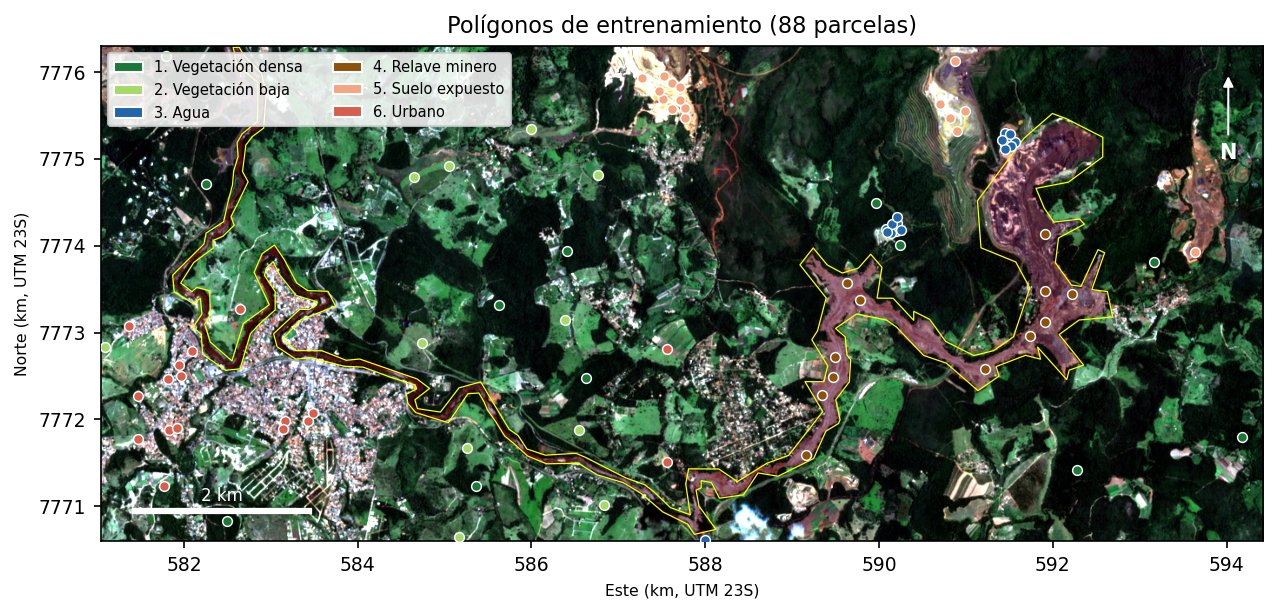
\includegraphics[width=\textwidth]{figures/poligonos_entrenamiento}
 \caption{Distribución de los polígonos de entrenamiento. Los puntos marcan el centro de cada parcela.}
 \label{fig:poligonos}
\end{figure}

\begin{figure}[htbp]
 \centering
 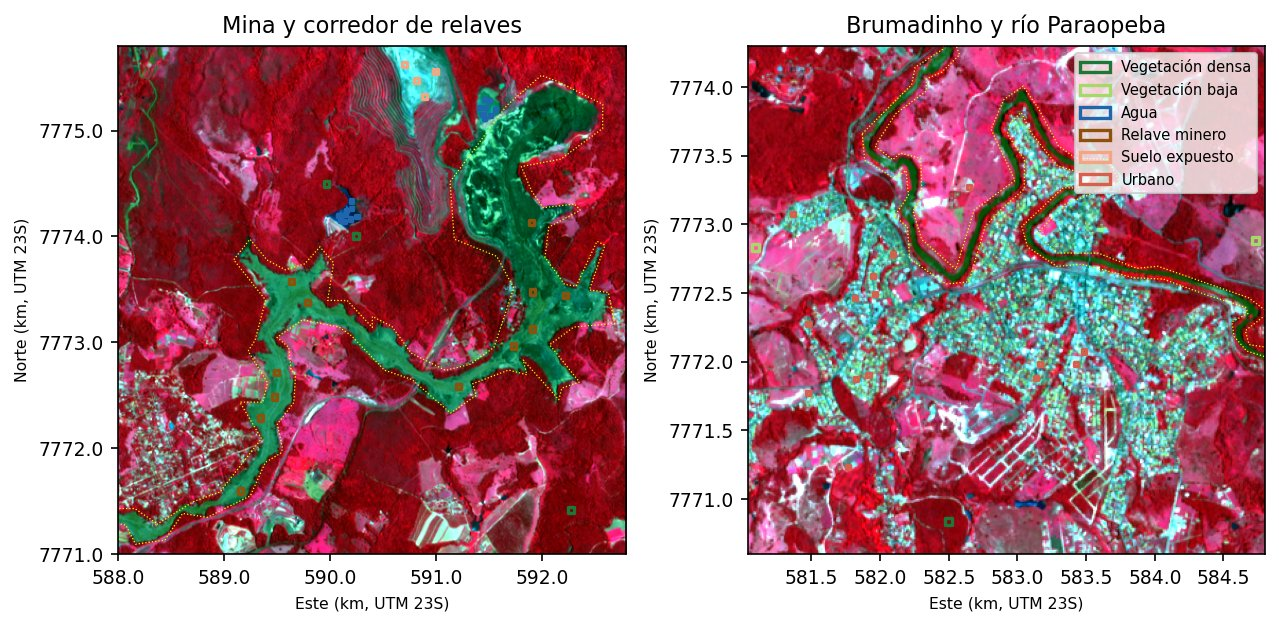
\includegraphics[width=\textwidth]{figures/poligonos_zoom}
 \caption{Detalle de los polígonos sobre la composición en falso color infrarrojo: corredor del relave (izquierda) y casco urbano de Brumadinho (derecha).}
 \label{fig:zoom}
\end{figure}

\subsection{Extracción de píxeles}
Los polígonos se rasterizan sobre la malla de la imagen, y se toma cada píxel cuyo centro cae dentro de un polígono. Se descartan los píxeles inválidos según la SCL y los que no tienen datos. Para cada píxel se calculan las coordenadas de su centro, que se transforman de UTM 23S a WGS84, y se leen los valores de las doce bandas.

Con estos datos se construye el archivo \texttt{training\_dataset.tsv}, separado por tabulaciones, en el que cada fila corresponde a un píxel. Sus columnas se describen en la Tabla~\ref{tab:columnas}, y la Tabla~\ref{tab:muestra} muestra un ejemplo por clase.

\begin{table}[htbp]
 \centering
 \caption{Estructura del archivo \texttt{training\_dataset.tsv} (17 columnas).}
 \label{tab:columnas}
 \begin{tabularx}{\textwidth}{lX}
  \toprule
  Columna & Contenido \\
  \midrule
  \texttt{Latitude}, \texttt{Longitude} & Centro del píxel en grados decimales (WGS84, EPSG:4326). \\
  \texttt{B01}--\texttt{B12} & Reflectancia de superficie $\times$ 10\,000 de las doce bandas (B01--B09, B8A, B11 y B12). \\
  \texttt{class\_id} & Código de la clase (1--6), igual al valor del ráster temático final. \\
  \texttt{class\_name} & Nombre de la clase. \\
  \texttt{poly\_id} & Identificador del polígono de origen. Permite separar entrenamiento y validación por polígono, de modo que píxeles vecinos no queden en ambos conjuntos. \\
  \bottomrule
 \end{tabularx}
\end{table}

\begin{table}[htbp]
 \centering
 \scriptsize
\setlength{\tabcolsep}{2.5pt}
 \caption{Primeras filas del TSV (una por clase).}
 \label{tab:muestra}
 \begin{tabular}{rrrrrrrrrrrrrrl}
  \toprule
  Lat & Lon & B01 & B02 & B03 & B04 & B05 & B06 & B07 & B08 & B8A & B09 & B11 & B12 & Clase \\
  \midrule
  -20{,}12967 & -44{,}17314 & 142 & 154 & 351 & 196 & 669 & 2087 & 2597 & 2632 & 2848 & 2824 & 1470 & 616 & Vegetacion densa \\
  -20{,}13681 & -44{,}17330 & 345 & 477 & 997 & 808 & 1708 & 2890 & 3190 & 3282 & 3509 & 3492 & 2656 & 1406 & Vegetacion baja \\
  -20{,}11796 & -44{,}12489 & 284 & 334 & 761 & 1074 & 1045 & 437 & 436 & 369 & 265 & 320 & 138 & 116 & Agua \\
  -20{,}12761 & -44{,}12054 & 301 & 296 & 416 & 656 & 783 & 865 & 879 & 772 & 806 & 850 & 1299 & 1184 & Relave minero \\
  -20{,}11380 & -44{,}16261 & 616 & 818 & 1450 & 2300 & 2526 & 2668 & 2602 & 2374 & 2316 & 2228 & 2750 & 2137 & Suelo expuesto \\
  -20{,}14857 & -44{,}21696 & 617 & 567 & 960 & 1814 & 1921 & 2314 & 2407 & 2472 & 2472 & 2403 & 3567 & 3211 & Urbano \\
  \bottomrule
 \end{tabular}
\end{table}


\subsection{Resumen del conjunto de datos}
La Tabla~\ref{tab:conteo} resume el número de polígonos y de píxeles por clase. El agua y el urbano siguen teniendo menos píxeles que la vegetación y el relave porque usan parcelas de $3 \times 3$ píxeles: los cuerpos de agua del área son estrechos y la zona urbana es heterogénea a 10\,m de resolución. La ampliación elevó el agua a 18 parcelas y el urbano a 17. Este desbalance se considerará en la Fase~2 mediante pesos por clase y el uso de métricas como F1 y Kappa, además de la exactitud global.

\begin{table}[htbp]
 \centering
 \caption{Polígonos y píxeles por clase en \texttt{training\_dataset.tsv}.}
 \label{tab:conteo}
 \begin{tabular}{clrrr}
  \toprule
  Código & Clase & Polígonos & Píxeles & \% \\
  \midrule
  1 & Vegetación densa & 12 & 300 & 18{,}3\,\% \\
  2 & Vegetación baja & 12 & 300 & 18{,}3\,\% \\
  3 & Agua & 18 & 162 & 9{,}9\,\% \\
  4 & Relave minero & 12 & 300 & 18{,}3\,\% \\
  5 & Suelo expuesto & 17 & 425 & 25{,}9\,\% \\
  6 & Urbano & 17 & 153 & 9{,}3\,\% \\
  \midrule
   & \textbf{Total} & 88 & 1640 & 100\,\% \\
  \bottomrule
 \end{tabular}
\end{table}


La Figura~\ref{fig:firmas} presenta la firma espectral por polígono (mediana e IQR entre polígonos) y muestra que las clases son, en general, separables:
\begin{itemize}
 \item las dos clases de vegetación presentan el aumento característico en el borde rojo (B05--B07) y se diferencian por su nivel en el infrarrojo cercano y en el SWIR;
 \item el agua tiene reflectancia baja en el infrarrojo cercano y en el SWIR;
 \item el relave muestra una firma plana, de nivel bajo a medio, distinta de la del suelo expuesto de la mina, que es más brillante en el visible y en el SWIR;
 \item las clases urbano y suelo expuesto son las más parecidas, por lo que es previsible que se confundan; esto justifica comparar modelos no lineales en la Fase~2.
\end{itemize}

\begin{figure}[htbp]
 \centering
 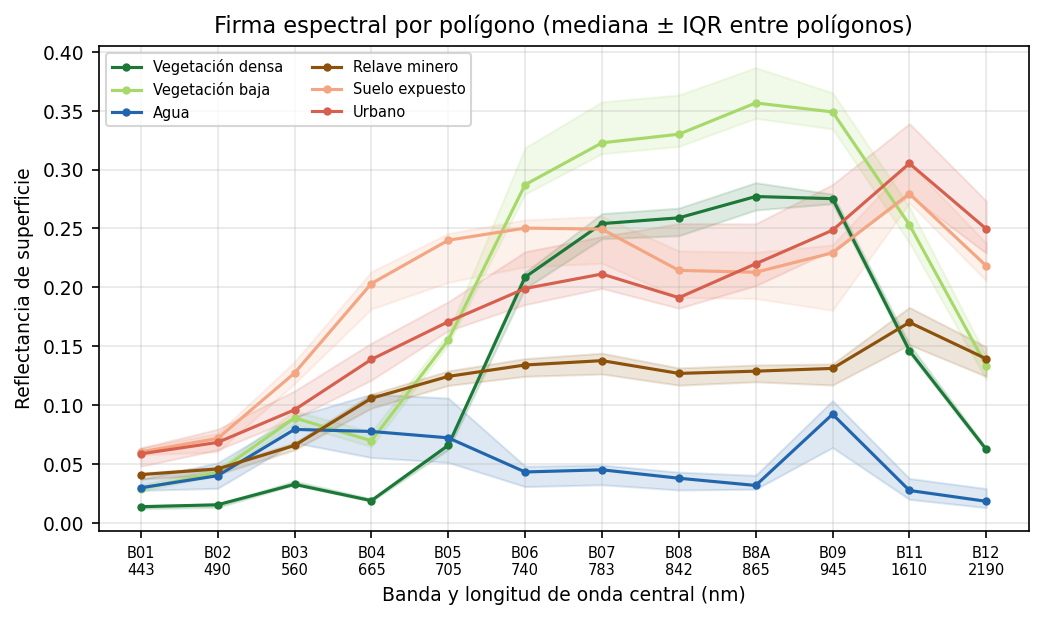
\includegraphics[width=0.85\textwidth]{figures/firmas_espectrales}
 \caption{Firma espectral por polígono: mediana e IQR entre polígonos de cada clase.}
 \label{fig:firmas}
\end{figure}

\subsection{Reproducibilidad}
La imagen de doce bandas, la capa SCL y los polígonos de entrenamiento se conservan como insumos del proyecto. A partir de ellos, el conjunto de datos y las figuras se generan con tres scripts de Python sobre un único entorno reproducible (\texttt{requirements.txt}), sin depender de QGIS (Tabla~\ref{tab:scripts}).

\begin{table}[htbp]
 \centering
 \caption{Scripts de la Fase 1.}
 \label{tab:scripts}
 \begin{tabularx}{\textwidth}{lX}
  \toprule
  Script & Función \\
  \midrule
  \texttt{01\_extract\_tsv.py} & Extrae los píxeles dentro de los polígonos y escribe el archivo TSV. \\
  \texttt{01b\_polygon\_dataset.py} & Agrega cada polígono (mediana, IQR e índices) y hace el control de calidad. \\
  \texttt{02\_figures.py} & Genera las figuras y tablas de este documento. \\
  \bottomrule
 \end{tabularx}
\end{table}

\section{Próximos pasos}
En la Fase~2 se dividirá el conjunto de datos en entrenamiento y prueba por polígono, se estandarizarán las bandas y se entrenarán los cinco modelos, reportando su matriz de confusión y su exactitud global. En la Fase~3 se optimizarán los hiperparámetros y se compararán los modelos con Kappa, precisión, exhaustividad y F1. Después, el mejor modelo se aplicará a toda la imagen para obtener el GeoTIFF temático y calcular el área de cada clase, en particular la superficie cubierta por el relave.

\printbibliography

\end{document}
